\section{Particle Physics}
To be able to understand the scope of the project and the applicability of the work in modern research, this chapter gives an overview of the key concepts from particle physics that appear through the paper. The explanation is written for readers with no prior background in physics.

\subsection{Standard Model}
the Standard Model is a theory that describes the connections between weak, strong and electromagnetic interactions, which are three of the fundamental forces. The possible unification with the forth one - gravity - is an ongoing research \cite{67-krasnov2018gravity}, and while certainly outside the scope of this project, it should be noted that some of the physical experiments that this work explores aim to help with it \cite{68-walz2015gbar,69-pagano2020gravity}.

The Standard Model also provides a classification of all the elementary particles. A non-exhaustive list of them is described below, with particles that this report is concerned about (as they appear in the proton-proton collisions) being highlighted.

\begin{itemize}[leftmargin=7mm]
  \item Fermions
  \begin{itemize}[leftmargin=5mm]
    \item Leptons - participate in electroweak interactions; include electron (e\textsuperscript{-})
    \item Quarks - participate in strong interactions; include \textbf{light quarks (q)}\footnote{Light flavor quarks: up (u), down (d), charm (c), and strange (s) quarks} and \textbf{top (t) quark}
  \end{itemize}
  \item Bosons
  \begin{itemize}[leftmargin=5mm]
    \item Gauge bosons - force carriers; include photon ($\gamma$), \textbf{W boson (W\textsuperscript{+}, W\textsuperscript{-})}, \textbf{Z boson}, \textbf{gluons}
    \item Scalar bosons - give rise to mass; include \textbf{Higgs boson (H\textsuperscript{0})}
  \end{itemize}
\end{itemize}

The information about the following decay processes form the dataset of this report, with visualization in figure \ref{fig:jedi-jets} (obtained from \cite{9-newman2019jedi-net:}). It is important to note that where applicable, the particles on the left-hand side of the arrows undergo a series of decays before reaching the right-hand side, when the only particles left are those composed of quarks and antiquarks (denoted by the vertical bar), referred to as hadrons.
\todo{Possibly clear page}
\[ q / g \]
\[ H^0 / W / Z \rightarrow q\overline{q} \]
\[ t \rightarrow Wq \rightarrow q\overline{q}q \]

\begin{figure}[hpt!]
  \centering
  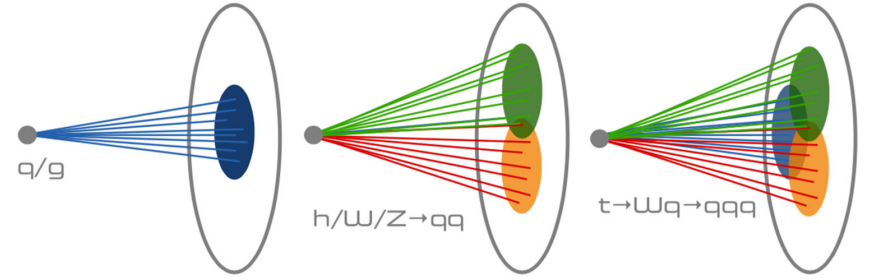
\includegraphics[trim={0cm 0cm 0cm 0cm}, width=0.6\textwidth, center]{background/jedi_jets.png}
  \caption{Representation of different decay processes, based on the number of resulting jet clusters.}
  \label{fig:jedi-jets}
\end{figure}

\subsection{Particle Accelerators and Triggers at LHC}\label{triggers}
The two LHC experiments that are of most concern in this report are CMS and ATLAS. They are both large general-purpose particle detectors, that were notably involved in the discovery of the Higgs boson \cite{47-greeene2013higgs}. Several processing steps happen between particles colliding and theories being proven, however real-time particle detectors comprises the very first elements of this pipeline. They are composed of triggers split into the following levels \citep[p.16]{48-trigger}:

\begin{itemize}
  \item \textbf{Level 1 trigger (L1T)} - it is implemented in hardware (FPGAs) and firmware, it is pipelined (a term explained in details in \autoref{serial-parallel-pipelined}) and it cannot allow for any dead-time, which means that it has to continuously process data with a fixed latency.
  \item \textbf{Level 2 trigger (L2T)} - it is implemented in hardware and software and can include regional processing.
  \item \textbf{Level 3 trigger (L3T)} - it is implemented in software, using farms of CPUs. It is close in behavior to non-real-time algorithms.
\end{itemize}

LHC operates in intertwined periods of operation and shutdown. The latter come from the demanding nature of the experiments that necessitates maintenance and upgrades to the apparatus and machinery, as well as the science and engineering advancements which allow for more efficient algorithms and technologies to be adopted. Very recently, after four years of break, LHC restarted experiments, which marks the beginning of "Run 3" \cite{70-keanecern's}. Since their origin, the L2T and L3T have been merged into High Level Trigger (HLT) \citep[p.47]{49-tappertriggering}, which is planned to rely on thousands of multithreaded CPUs and GPUs. As for the L1T key specifications that will be used to evaluate the design in this paper, its input data frequency is 40 MHz, which with a pipeline depth of 500 results in a 12.5 \(\mu s\) latency, and its output frequency to HLT is equal to 750 kHz.

\subsection{Dataset and Notations}
The datasets used in this work has been simulated to mimic the 13 TeV proton-proton collisions performed at LHC, and it includes information about the most energetic jets \cite{61-coleman2018importance} (30 \cite{31-pierinihls4ml}, 50 \cite{32-pierinihls4ml}, 100 \cite{33-pierinihls4ml} and 150 \cite{34-pierinihls4ml}) that were constructed using the anti-K\textsubscript{t} clustering algorithm \cite{35-cacciari2008anti-kt}. A number of jet representations are available in the dataset:

\begin{itemize}
  \item High level features (HLF), which are physically inspired,
  \item Images, which are related to an energy heat-map,
  \item Constituent list, which contains jets' constituent hadrons from the following list: light quarks, top quarks, W bosons, Z bosons, and gluons.
\end{itemize}

Compared to the other two, the constituent list is a lower-level representation, however, as mentioned in \cref{introduction}, this should not affect the classification accuracy \cite{7-moore2019reports}. It is also worth mentioning that a simpler dataset that contains only the HLF jet representation \cite{36-kreinar2018fast} is also used in this project as it vastly reduces the complexity of a design while offering comparable accuracy. A more thorough discussion between the differences in their use cases is carried in \cref{evaluation}, but it is worth mentioning that the HLF representation has been successfully used in conjunction with deep neural networks \cite{53-kreinar2018fast}, while the images and constituent lists were adopted for graph neural networks \cite{9-newman2019jedi-net:}.

To facilitate further analysis, this subsection also explains the notation used for the dataset as it is important throughout the report. Each constituent element \(\bm{x^l}\) is a 16-dimensional vector, where \(l\) denotes the index in the list:

\begin{equation}
  \bm{x^l} =
  \begin{bmatrix}
    x^l_{0} & x^l_{1} & \hdots & x^l_{15}
  \end{bmatrix}^T \in \mathbb{R}^{16}
\end{equation}

The physical meaning of each element's dimension is not taken into consideration, and all of them are treated as equally important. A constituent list \(\bm{x^i}\) acts a single sample, with index \(i\) within a dataset, and it varies in terms of the number of constituents \(L\), but it has no more of them than the dataset name suggests:

\begin{equation}
  \bm{\hat{x^i}} =
  \begin{bmatrix}
    \bm{x^{i,0}} & \bm{x^{i,1}} & \hdots & \bm{x^{i,L-1}}
  \end{bmatrix} \in \mathbb{R}^{L \times 16}
\end{equation}

Using the 30 jet dataset as an example, each sample has between 1 and 30 constituents, although in the majority of samples it is the upper boundary. Hence, the whole dataset with \(N\) samples can be represented as \(D\):

\begin{equation}
  D =
  \begin{bmatrix}
    \bm{\hat{x^0}} \\
    \bm{\hat{x^1}} \\
    \vdots \\
    \bm{\hat{x^{N-1}}}
  \end{bmatrix} =
  \begin{bmatrix}
    \bm{x^{0,0}} & \bm{x^{0,1}} & \hdots & \bm{x^{0,L-1}} \\
    \bm{x^{1,0}} & \bm{x^{1,1}} & \hdots & \bm{x^{1,L-1}} \\
    \vdots & \vdots & \ddots & \vdots \\
    \bm{x^{N-1,0}} & \bm{x^{N-1,1}} & \hdots & \bm{x^{N-1,L-1}} \\
  \end{bmatrix} \in \mathbb{R}^{N \times L \times 16}
\end{equation}

The main jet datasets contain \(880,000\) samples regardless of the number of jets per sample, while the HLF dataset contains \(830,000\) examples, which are split into training and test samples in \(70:30\) and \(80:20\) proportions accordingly. In both cases, the datasets are balanced, meaning that they contain all available particle classes in near identical proportions. This is a desired characteristic of data as it avoids having to introduce weighted results as a measure of protecting the model from not learning the underrepresented classes properly. When it comes to the distribution and range of values for each feature, the visualizations can be seen in figure \ref{fig:distributions-hlf}\maybe{Maybe city the OpenML website} and TODO for HLF and constituent list datasets respectively.

\begin{figure}[hpt!]
  \centering
  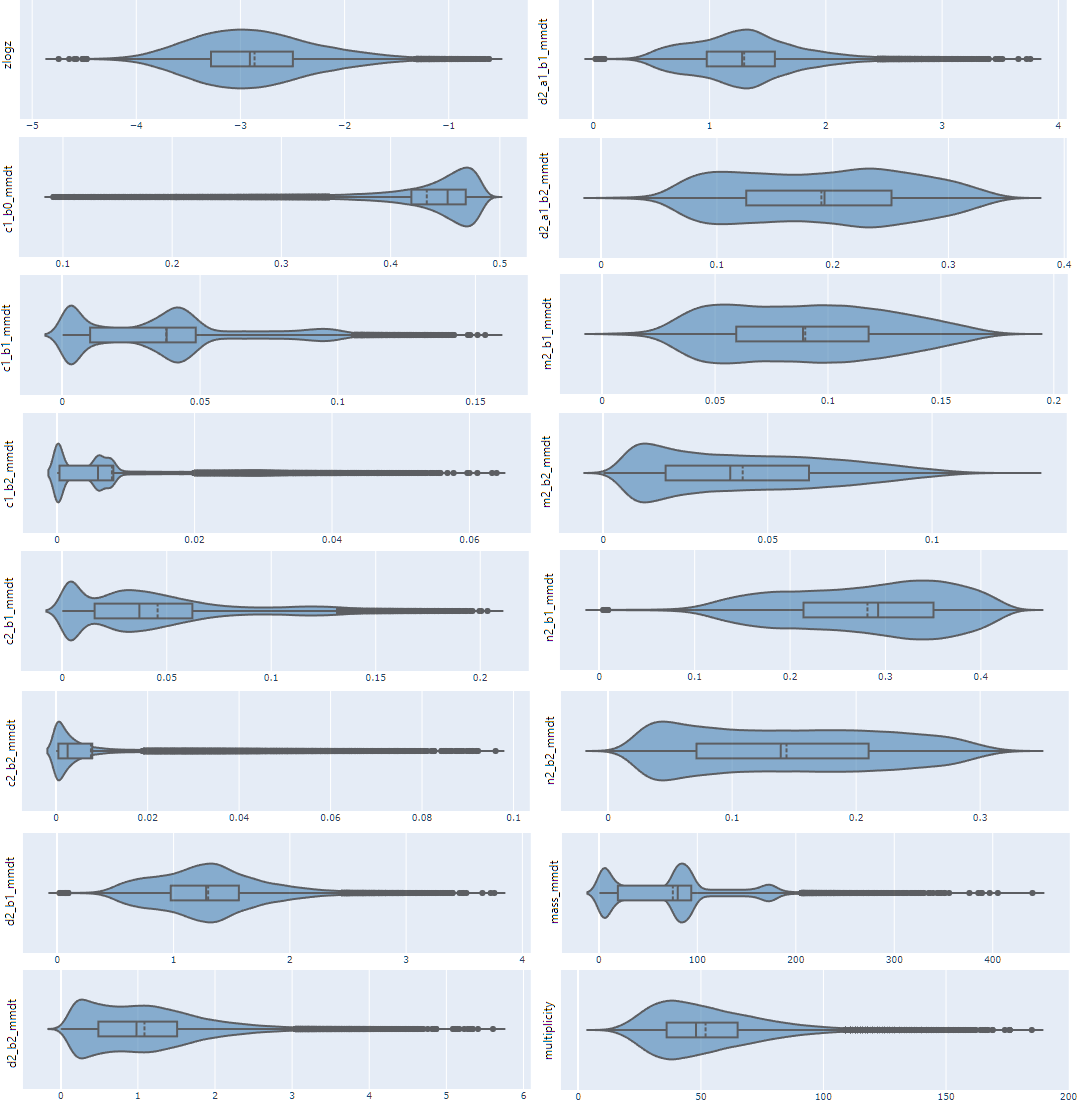
\includegraphics[trim={0cm 0cm 0cm 0cm}, width=1.0\textwidth, center]{background/distributions.png}
  \caption{Representation of the distributions of feature values in the HLF dataset.}
  \label{fig:distributions-hlf}
\end{figure}

It is also worth mentioning that normalization\footnote{Process of subtracting mean and dividing by standard deviation, also referred to as "standardization".} is the only preprocessing measure used in this work, and it is only applied to the HLF dataset. The reasons behind avoiding it in case of the constituent list dataset are discussed in detail in \cref{accuracy-focused-model}. Both dataset samples are simulated and do not contain any illegal or null values that would require dropping or substituting. There is also no need for data augmentation because of the simulated origin of data.

\todofig{Constituent list feature distribution}
\todofig{|}
\todofig{|}
\todofig{|}
\todofig{|}
\todofig{|}
\todofig{|}
\todofig{|}
